\documentclass[xcolor=x11names,t,aspectratio=169]{beamer}

% ---------------- TEMPLATE / COLORS ----------------
\IfFileExists{Cmd.tex}{% ---------------- PACKAGES ----------------
\usepackage[utf8]{inputenc}
\usepackage[T1]{fontenc}
\usepackage{lmodern}
\usepackage{booktabs}
\usepackage{array}
\usepackage{tabularx}
\usepackage{xcolor}
\usepackage{array}
\usepackage{tikz}
\usepackage{amssymb}
\usepackage{appendixnumberbeamer}
\usetikzlibrary{arrows.meta,positioning,shapes.geometric,fit,calc,decorations.pathmorphing, positioning,shapes.symbols}
\usepackage{enumitem}
% ---------------- COLORS ----------------
\definecolor{gravyblue}{RGB}{0,59,105}
\definecolor{deepblue}{RGB}{0,45,85}
\definecolor{softblue}{RGB}{231,242,249}
\definecolor{midblue}{RGB}{0,105,170}
\definecolor{tealblue}{RGB}{0,136,150}
\definecolor{softgray}{RGB}{245,247,250}
\definecolor{darkgray}{RGB}{60,70,80}
\definecolor{alertred}{RGB}{184,40,55}
\definecolor{warmgold}{RGB}{235,170,60}

\usecolortheme[named=gravyblue]{structure}

\setbeamercolor{frametitle}{bg=gravyblue, fg=white}
\setbeamercolor{title}{fg=white}
\setbeamercolor{title in head/foot}{bg=softblue, fg=gravyblue}
\setbeamercolor{author in head/foot}{bg=gravyblue, fg=white}
\setbeamercolor{date in head/foot}{bg=deepblue, fg=white}
\setbeamercolor{normal text}{fg=darkgray,bg=white}
\setbeamercolor{block title}{bg=gravyblue,fg=white}
\setbeamercolor{block body}{bg=softblue,fg=darkgray}

\setbeamertemplate{block begin}{
  \par\vskip\medskipamount
  \begin{beamercolorbox}[colsep*=.75ex,center]{block title}
    \usebeamerfont*{block title}\insertblocktitle
  \end{beamercolorbox}
  {\parskip0pt\par}
  \begin{beamercolorbox}[colsep*=.75ex,vmode]{block body}
    \usebeamerfont{block body}
}

\setbeamertemplate{navigation symbols}{}
\setbeamertemplate{caption}[numbered]

% Numbered table of contents
\setbeamertemplate{itemize item}{\color{gravyblue}$\bullet$}
\setbeamertemplate{itemize subitem}{\color{gravyblue}$\circ$}
\setbeamertemplate{itemize subsubitem}{\color{gravyblue}$-$}

\setlist[itemize,1]{
  label=\textcolor{gravyblue}{$\bullet$},
  leftmargin=1.5em
}

\setlist[itemize,2]{
  label=\textcolor{gravyblue}{$\circ$},
  leftmargin=1.5em
}

\setlist[itemize,3]{
  label=\textcolor{gravyblue}{$-$},
  leftmargin=1.5em
}
% ---------- Citation color ----------
\hypersetup{
    colorlinks=true,
    linkcolor=gravyblue,
    citecolor=gravyblue,
    urlcolor=gravyblue
}


% ---------------- LOGOS ----------------
\newcommand{\safelogo}[2]{%
  \IfFileExists{#2}{\includegraphics[height=#1,keepaspectratio]{#2}}{}%
}

\logo{\safelogo{0.75cm}{figures/ece.png}}

% ---------------- FOOTER ----------------
\setbeamertemplate{footline}{%
  \leavevmode%
  \hbox{%
  \begin{beamercolorbox}[wd=.27\paperwidth,ht=3ex,dp=1ex,center,sep=0pt]{author in head/foot}%
    \usebeamerfont{author in head/foot}\insertshortauthor
  \end{beamercolorbox}%
  \begin{beamercolorbox}[wd=.51\paperwidth,ht=3ex,dp=1ex,center,sep=0pt]{title in head/foot}%
    \usebeamerfont{title in head/foot}\insertshorttitle
  \end{beamercolorbox}%
  \begin{beamercolorbox}[wd=.22\paperwidth,ht=3ex,dp=1ex,center,sep=0pt]{date in head/foot}%
    \usebeamerfont{date in head/foot}\insertframenumber/\inserttotalframenumber
  \end{beamercolorbox}}%
}


% ---------------- HELPERS ----------------
\newcommand{\sectiondivider}[2]{%
\begin{frame}[plain]
\begin{tikzpicture}[remember picture,overlay]
  \fill[gravyblue] (current page.south west) rectangle (current page.north east);
  \fill[softblue,opacity=.14] ($(current page.north west)+(0,-1.3)$) circle (3.2);
  \fill[midblue,opacity=.18] ($(current page.south east)+(-1.0,0.6)$) circle (3.6);
\end{tikzpicture}
\vspace{1.5cm}
\begin{center}
{\color{white}\Huge\bfseries #1}\\[0.4cm]
{\color{softblue}\Large #2}
\end{center}
\end{frame}
}


\newcommand{\pill}[1]{%
\tikz[baseline=(X.base)] \node[fill=softblue,draw=midblue,rounded corners=5pt,inner xsep=7pt,inner ysep=3pt] (X) {\small\bfseries\color{gravyblue} #1};%
}

\providecommand{\framewithtitle}[1]{\sectiondivider{#1}{}}

% ---------------- CUSTOM TITLE PAGE ----------------
\setbeamertemplate{title page}{
\vspace*{0.18cm}
\begin{center}
\begin{minipage}{0.95\linewidth}
\centering
\safelogo{1.55cm}{figures/CNAM.jpg}
\hspace{0.8cm}
\safelogo{1.55cm}{figures/ece.png}
\hspace{0.8cm}
\raisebox{0.3cm}{\safelogo{0.95cm}{figures/cedric.png}}
\end{minipage}

\vspace{0.22cm}

\begin{beamercolorbox}[
    wd=0.9\paperwidth,
    rounded=true,
    shadow=true,
    sep=0.42cm,
    center
]{frametitle}
{\usebeamerfont{title}\LARGE\bfseries\inserttitle}
\end{beamercolorbox}

\vspace{0.25cm}
{\Large\bfseries \insertauthor}

\vspace{0.2cm}
{\large \insertinstitute}

% \vspace{0.18cm}
% {\large \insertdate}
\end{center}
}

% -------- Timeline colors --------
\definecolor{gravyblue}{RGB}{0,59,105}
\definecolor{midblue}{RGB}{0,92,150}
\definecolor{softblue}{RGB}{229,241,250}
\definecolor{verysoftblue}{RGB}{245,250,253}
\definecolor{lineblue}{RGB}{70,130,180}

\tikzset{
    timelinebox/.style={
        draw=gravyblue,
        very thick,
        rounded corners=2pt,
        align=center,
        font=\scriptsize\bfseries,
        inner sep=2.5pt,
        text=black
    },
    edu/.style={
        timelinebox,
        fill=verysoftblue
    },
    scholar/.style={
        timelinebox,
        fill=softblue
    },
    award/.style={
        timelinebox,
        fill=white
    },
    activity/.style={
        timelinebox,
        fill=softblue!65
    },
    sectionbg/.style={
        draw=lineblue,
        thick,
        rounded corners=2pt,
        fill=softblue!35
    },
    sectiontitle/.style={
        font=\small\bfseries,
        text=gravyblue
    },
    ylabel/.style={
        font=\small\bfseries,
        text=gravyblue,
        align=center
    }
}
\tikzset{
  boxbase/.style={
    draw=gravyblue,
    thick,
    rounded corners=2pt,
    align=center,
    inner sep=2.5pt,
    font=\scriptsize
  },
  edu/.style={boxbase, fill=white},
  scholar/.style={boxbase, fill=softblue!20},
  award/.style={boxbase, fill=white},
  activity/.style={boxbase, fill=softblue!35},
  sectionbg/.style={
    draw=midblue!75,
    thin,
    rounded corners=2pt,
    fill=softblue!10
  },
  sectiontitle/.style={
    font=\small\bfseries,
    text=gravyblue
  },
  ylabel/.style={
    font=\small\bfseries,
    text=gravyblue
  }
}
% -------- Alert box --------
\setbeamercolor{block title alerted}{bg=red!75!black, fg=white}
\setbeamercolor{block body alerted}{bg=red!8, fg=black}

% ---------- Diagram Methods Styles ----------
\definecolor{pblue}{RGB}{53,104,191}
\definecolor{pgreen}{RGB}{103,154,103}
\definecolor{ppurple}{RGB}{125,88,170}
\definecolor{pyellow}{RGB}{226,184,24}
\definecolor{boxbg}{RGB}{250,250,250}
\definecolor{textdark}{RGB}{55,65,75}

\tikzset{
  phasearrow/.style={
    signal,
    signal from=west,
    signal to=east,
    line width=1.15pt,
    fill=boxbg,
    minimum height=1.25cm,
    align=center,
    font=\bfseries\large,
    text=textdark,
    inner sep=2pt
  },
  methodbox/.style={
    rounded corners=0.18cm,
    line width=1.15pt,
    fill=white,
    align=left,
    anchor=north,
    inner sep=0.25cm,
    font=\scriptsize,
    text=textdark
  },
  boxtitle/.style={
    font=\bfseries\small,
    text=textdark
  },
  keylabel/.style={
    font=\bfseries,
    text=textdark
  }
}}{%
  \usetheme{Madrid}
  \usecolortheme{whale}
}
\providecolor{gravyblue}{RGB}{24,54,90}
\providecolor{softblue}{RGB}{214,229,245}
\providecolor{midblue}{RGB}{47,98,151}
\providecolor{tealblue}{RGB}{40,120,135}
\providecolor{softgray}{RGB}{240,240,240}
\providecolor{alertred}{RGB}{176,42,42}
\usepackage{amsmath,amssymb}
\usepackage{tikz}
\usetikzlibrary{shadows,positioning,arrows.meta,calc,shapes.geometric,fit}

% ---- Figure colours: same as the article (red = class 0, green = class 1) ----
\definecolor{cHigh}{HTML}{D62728}
\definecolor{cLow}{HTML}{2CA02C}
\definecolor{cReq}{HTML}{1F77B4}
\definecolor{cNode}{HTML}{EEF3FA}
\definecolor{cSwitch}{HTML}{E8E8E8}
\tikzset{
  es/.style={ellipse, draw=black!70, fill=cNode, minimum width=0.8cm, minimum height=0.4cm, inner sep=0pt, drop shadow={opacity=0.2}},
  sw/.style={rectangle, rounded corners=3pt, draw=black!70, fill=cSwitch, minimum width=0.85cm, minimum height=0.42cm, drop shadow={opacity=0.2}},
  link/.style={{Latex[length=1.5mm]}-{Latex[length=1.5mm]}, thick, black!75},
  route/.style={-{Latex[length=2mm]}, thick, rounded corners=5pt},
  pkt/.style={draw=black!70, line width=0.3pt, minimum height=0.3cm, inner sep=0pt},
  flow/.style={-{Stealth[length=1.9mm, width=1.6mm]}, line width=0.8pt, line cap=round, shorten <=1.5pt, shorten >=1pt},
  box/.style={rectangle, rounded corners=3pt, draw=black!70, align=center, minimum height=0.55cm, drop shadow={opacity=0.2}},
  data/.style={rectangle, rounded corners=2pt, draw=black!60, dashed, align=center, fill=white, minimum height=0.55cm},
}

\setbeamertemplate{navigation symbols}{}
\setbeamertemplate{itemize items}[circle]

% ---- Key-number tile: \stattile{colour}{number}{caption} ----
\newcommand{\stattile}[3]{%
  \tikz[baseline]\node[rounded corners=4pt, fill=#1!10, draw=#1!70, line width=0.8pt,
    minimum width=3.2cm, minimum height=1.05cm, align=center, inner sep=3pt, drop shadow={opacity=0.15}]
    {{\large\bfseries\color{#1}#2}\\[1pt]{\scriptsize #3}};}

% ---------------- TITLE INFO ----------------
\title[A Certified Admission Gate for TSN]{A Certified Admission Gate for Online Reconfiguration of Time-Sensitive Networks}

\author[Le Huyen-Trang]{
{\normalsize Huyen-Trang Le, Computer Network Master Program -- M2 CNS SR}\\[0.08cm]
{\scriptsize Under the supervision of Dr. Aakash Soni and Prof. Samia Saad-Bouzefrane}
}

\institute[LyRIDS (ECE) -- CEDRIC (Cnam)]{
\footnotesize Preparatory work for the PhD thesis \textit{Certified Dynamic Reconfiguration of Time-Sensitive Networks:\\Online Admission Control under Worst-Case Determinism Guarantees}\\[0.05cm]
\textbf{PhD Thesis Proposal in LyRIDS (ECE) / CEDRIC (Cnam), Paris}
}
\date{}

\begin{document}

\begin{frame}[plain]
\titlepage
\end{frame}

\begin{frame}{Outline}
\vspace{-0.2cm}
\tableofcontents
\end{frame}

% ============================================================
\section{1. Problem}
% ============================================================

\begin{frame}{1. Problem: Worst-Case Guarantees in a Changing Network}
\small
\begin{block}{Context}
Factories, vehicles and aircraft replace dedicated fieldbuses with \textbf{one Ethernet network} shared by control loops, sensors, video and best-effort traffic. For control traffic, a late message is \textbf{a failure}, not a slower service: what is needed is a \textbf{guaranteed worst case}.
\end{block}
\begin{itemize}
  \item \textbf{TSN} (IEEE 802.1Q \cite{ieee8021q}) gives bounded latency, but only for a flow set \textbf{analysed offline}, with network calculus \cite{cruz1991calculus,leboudec2001nc} or a synthesised schedule \cite{xue2024tsn}.
  \item In operation, \textbf{flows are added while the network runs}; each new flow can delay flows already admitted, \textbf{even on other paths} that share a port.
  \item Fast \textbf{proposers} exist (heuristics, ILP/SMT, deep RL), but their outputs are \textbf{optimised, not proven}.
\end{itemize}
\vspace{0.1cm}
\begin{center}
\pill{After this change, does every admitted flow still meet its deadline?}
\end{center}
\end{frame}

\begin{frame}{1. Problem: Our Approach and Contributions}
\small
\begin{columns}[T,totalwidth=\textwidth]
\column{0.55\textwidth}
\begin{block}{A certified admission gate}
Placed between \textbf{any} proposer and the network, like a safety shield \cite{alshiekh2018shield}: a change is committed only with a \textbf{certificate} that an \textbf{independent checker} re-verifies.
\end{block}
\begin{itemize}
  \item \textbf{C1.} Gate $\mathrm{admit}(S,f)\to(\mathit{verdict},\mathit{certificate})$ for non-preemptive static-priority TSN, with a soundness argument.
  \item \textbf{C2.} Incremental gate: recomputes only the affected ports, \textbf{bit-identical} bounds.
  \item \textbf{C3.} Validation against \textbf{panco} \cite{bouillard2022panco}, simulation and tests; fully reproducible.
  \item \textbf{C4.} Explicit limits of the guarantee.
\end{itemize}
\column{0.42\textwidth}
\centering
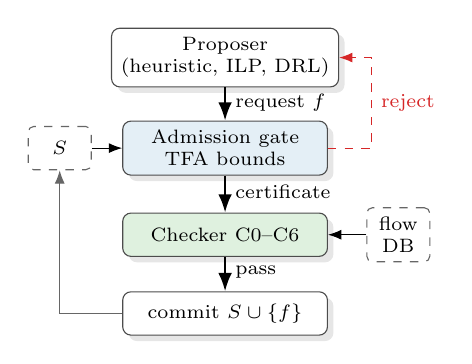
\begin{tikzpicture}[font=\scriptsize, >=Latex]
  \node[box, minimum width=2.6cm, fill=white] (prop) at (1.9, 3.0) {Proposer\\(heuristic, ILP, DRL)};
  \node[box, minimum width=2.6cm, fill=cReq!12] (gate) at (1.9, 1.85) {Admission gate\\TFA bounds};
  \node[box, minimum width=2.6cm, fill=cLow!15] (chk) at (1.9, 0.75) {Checker C0--C6};
  \node[box, minimum width=2.6cm, fill=white] (com) at (1.9, -0.25) {commit $S \cup \{f\}$};
  \node[data, minimum width=0.8cm] (st) at (-0.2, 1.85) {$S$};
  \node[data, minimum width=0.8cm] (db) at (4.1, 0.75) {flow\\DB};
  \draw[->, thick] (prop) -- node[right, pos=0.45] {request $f$} (gate);
  \draw[->, thick] (gate) -- node[right, pos=0.45] {certificate} (chk);
  \draw[->, thick] (chk) -- node[right, pos=0.45] {pass} (com);
  \draw[->] (st) -- (gate);
  \draw[->] (db) -- (chk);
  \draw[->, black!60] (com.west) -| (st.south);
  \draw[->, dashed, cHigh] (gate.east) -- ++(0.55, 0) |- node[right, pos=0.25] {reject} (prop.east);
\end{tikzpicture}
\end{columns}
\end{frame}

% ============================================================
\section{2. Model}
% ============================================================

\begin{frame}{2. Model: Network, Flows and Scheduling}
\small
\begin{columns}[T,totalwidth=\textwidth]
\column{0.5\textwidth}
\begin{itemize}
  \item \textbf{Network}: switches and end stations, full-duplex links of rate $C=1$\,Gbit/s; each link direction is an output \textbf{port}; processing delay $t_{proc}$.
  \item \textbf{Routing}: fixed shortest paths; port dependency graph checked \textbf{feed-forward}.
  \item \textbf{Flow} $f$: token bucket $\alpha_f(t)=b_f+r_f t$, max frame $L_f$, priority class $k_f$ (0 highest), deadline $D^{\max}_f$.
  \item \textbf{Ports}: non-preemptive static priority (\textbf{NP-SP}), FIFO within a class.
\end{itemize}
\column{0.48\textwidth}
\centering
\vspace{0.2cm}
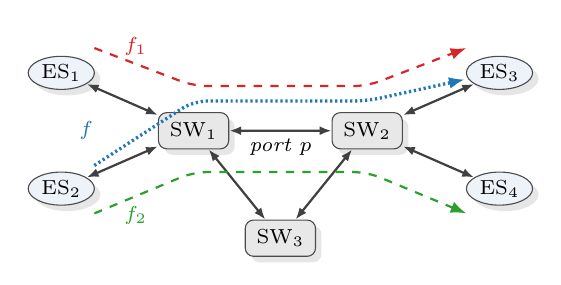
\begin{tikzpicture}[font=\scriptsize, >=Latex, scale=1.05, transform shape]
  \node[es] (es1) at (0, 1.9) {ES$_1$};
  \node[es] (es2) at (0, 0.5) {ES$_2$};
  \node[sw] (sw1) at (1.6, 1.2) {SW$_1$};
  \node[sw] (sw2) at (3.7, 1.2) {SW$_2$};
  \node[es] (es3) at (5.3, 1.9) {ES$_3$};
  \node[es] (es4) at (5.3, 0.5) {ES$_4$};
  \node[sw] (sw3) at (2.65, -0.1) {SW$_3$};
  \foreach \a/\b in {es1/sw1, es2/sw1, sw1/sw2, sw2/es3, sw2/es4, sw1/sw3, sw2/sw3}
    \draw[link] (\a) -- (\b);
  \draw[route, cHigh, dashed] (0.4, 2.2) -- (1.6, 1.74) -- (3.7, 1.74) -- (4.9, 2.2);
  \draw[route, cReq, densely dotted, very thick] (0.4, 0.78) -- (1.6, 1.56) -- (3.7, 1.56) -- (4.88, 1.82);
  \draw[route, cLow, dashed] (0.4, 0.2) -- (1.6, 0.7) -- (3.7, 0.7) -- (4.9, 0.2);
  \node[cHigh] at (0.9, 2.22) {$f_1$};
  \node[cReq]  at (0.3, 1.2) {$f$};
  \node[cLow]  at (0.9, 0.18) {$f_2$};
  \node[font=\scriptsize\itshape] at (2.65, 1.0) {port $p$};
\end{tikzpicture}

\vspace{0.15cm}
{\scriptsize Admitted $f_1$ (class 0), $f_2$ (class 1) and a new class-0 request $f$ share port $p$: admitting $f$ can delay both.}
\end{columns}
\end{frame}

\begin{frame}{2. Model: Packet Handling and Delay Bounds at an NP-SP Port}
\small
\begin{columns}[T,totalwidth=\textwidth]
\column{0.5\textwidth}
\centering
\vspace{0.3cm}
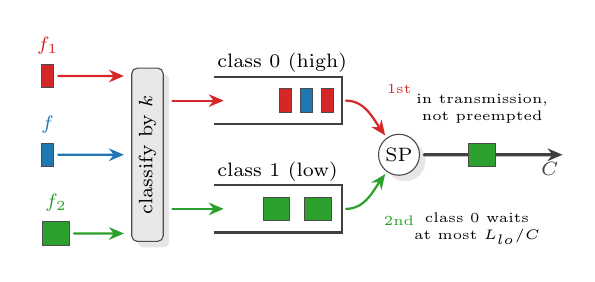
\begin{tikzpicture}[font=\scriptsize, >=Latex, xscale=1.32, yscale=1.25]
  \node[pkt, fill=cHigh, minimum width=0.15cm] (a1) at (0.12, 2.05) {};
  \node[pkt, fill=cReq,  minimum width=0.15cm] (a2) at (0.12, 1.25) {};
  \node[pkt, fill=cLow,  minimum width=0.34cm] (a3) at (0.2, 0.45) {};
  \foreach \n/\y/\c in {a1/2.05/cHigh, a2/1.25/cReq, a3/0.45/cLow} \draw[flow, \c] (\n.east) -- (0.88, \y);
  \node[cHigh] at (0.12, 2.36) {$f_1$};
  \node[cReq]  at (0.12, 1.56) {$f$};
  \node[cLow]  at (0.2, 0.76) {$f_2$};
  \node[rectangle, rounded corners=2pt, draw=black!70, fill=cSwitch, minimum width=0.4cm, minimum height=2.2cm, drop shadow={opacity=0.2}] at (1.08, 1.25) {};
  \node[rotate=90] at (1.08, 1.25) {classify by $k$};
  \foreach \y/\lab/\c in {1.8/class 0 (high)/cHigh, 0.7/class 1 (low)/cLow} {
    \draw[thick, black!75] (1.72, \y+0.24) -- (2.95, \y+0.24) -- (2.95, \y-0.24) -- (1.72, \y-0.24);
    \node[anchor=south west, inner sep=1pt] at (1.72, \y+0.25) {\lab};
    \draw[flow, \c] (1.28, \y) -- (1.84, \y);
  }
  \node[pkt, fill=cHigh, minimum width=0.15cm] at (2.81, 1.8) {};
  \node[pkt, fill=cReq,  minimum width=0.15cm] at (2.61, 1.8) {};
  \node[pkt, fill=cHigh, minimum width=0.15cm] at (2.41, 1.8) {};
  \node[pkt, fill=cLow,  minimum width=0.34cm] at (2.72, 0.7) {};
  \node[pkt, fill=cLow,  minimum width=0.34cm] at (2.32, 0.7) {};
  \node[circle, draw=black!70, fill=white, minimum size=0.52cm, inner sep=0pt, drop shadow={opacity=0.2}] (sp) at (3.5, 1.25) {SP};
  \draw[flow, cHigh] (2.95, 1.8) to[out=0, in=125] (sp);
  \draw[flow, cLow]  (2.95, 0.7) to[out=0, in=235] (sp);
  \node[cHigh, font=\tiny] at (3.5, 1.92) {1st};
  \node[cLow,  font=\tiny] at (3.5, 0.58) {2nd};
  \draw[flow, black!75, line width=1.1pt] (sp.east) -- (5.1, 1.25) node[below left, inner sep=2pt] {$C$};
  \node[pkt, fill=cLow, minimum width=0.34cm] at (4.3, 1.25) {};
  \node[align=center, font=\tiny] at (4.3, 1.72) {in transmission,\\not preempted};
  \node[align=center, font=\tiny] at (4.25, 0.5) {class 0 waits\\at most $L_{lo}/C$};
\end{tikzpicture}
\column{0.47\textwidth}
\begin{block}{Per-hop bound for class $k$ at port $p$}
{\footnotesize Residual rate-latency service \cite{leboudec2001nc,bouillard2018dnc}:}
\vspace{-0.2cm}
\[
d_k=\frac{B_H+L_{lo}+B_k}{C-R_H}+t_{proc},\qquad R_H+R_k\le C
\]
\vspace{-0.4cm}
\end{block}
\begin{block}{Burst propagation and end-to-end bound (TFA)}
\vspace{-0.2cm}
\[
b'=b+r_f\,d_k,\qquad D_f=\sum_{h\in\mathcal{P}_f} d_{k_f}^{(h)}\le D^{\max}_f
\]
\vspace{-0.4cm}
\end{block}
{\footnotesize $B_H,R_H$: higher-priority bursts and rates; $L_{lo}$: largest lower-priority frame (non-preemptive blocking); $B_k,R_k$: class-$k$ aggregates.}
\end{columns}
\end{frame}

% ============================================================
\section{3. Admission Gate}
% ============================================================

\begin{frame}{3. Admission Gate: Certificate and Independent Checker}
\small
\begin{columns}[T,totalwidth=\textwidth]
\column{0.46\textwidth}
\begin{block}{Interface and invariant}
On request $f$, analyse $S\cup\{f\}$; accept iff it is schedulable. \textbf{Invariant}: every flow in $S$ meets its deadline. A rejection lists \textbf{every} violated flow, not only $f$.
\end{block}
\begin{block}{Certificate}
Per flow: path and, per hop, $b_{in}$, $(B_H,R_H,L_{lo},B_k,R_k)$, $d$; end-to-end bound; fingerprint of $S$ before/after (XOR of SHA-256 flow hashes).
\end{block}
\column{0.51\textwidth}
\begin{block}{Checker (about fifty lines, no analysis code)}
\footnotesize
\begin{itemize}
  \item[C0] one witness per admitted flow, with its own parameters
  \item[C1] each path is the fixed route
  \item[C2] first input burst $\ge b_f$
  \item[C3] next input burst $\ge b_{in}+r_f d$
  \item[C4] claimed aggregates $\ge$ those recomputed from all witnesses at the port
  \item[C5] $R_H<C$, $R_H+R_k\le C$, $d\ge$ per-hop bound
  \item[C6] end-to-end bound $\ge\sum d$ and $\le$ deadline
\end{itemize}
\end{block}
\end{columns}
\end{frame}

\begin{frame}{3. Admission Gate: Soundness and Incremental Computation}
\small
\begin{block}{Proposition (soundness)}
If a certificate passes C0--C6, every admitted flow meets its deadline under the model.
\end{block}
\vspace{0.15cm}
\begin{columns}[T,totalwidth=\textwidth]
\column{0.47\textwidth}
\textcolor{gravyblue}{\textbf{Why it holds}}
\footnotesize
\begin{itemize}
  \item The bound grows with $B_H,R_H,L_{lo},B_k$.
  \item Induction over the \textbf{topological order of ports}: every witnessed burst over-approximates the true one (C2--C5).
  \item Summing the hops gives the deadline (C6).
  \item \textbf{C0 is necessary}: omitting a flow only \emph{lowers} the others' aggregates; only the flow database reveals it.
\end{itemize}
\column{0.5\textwidth}
\centering
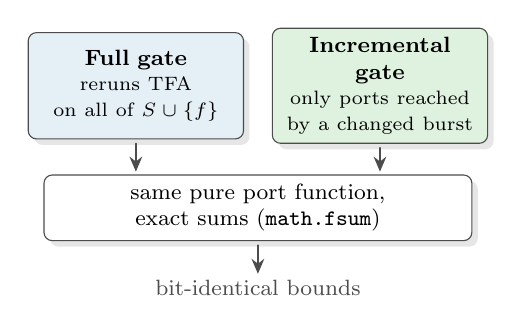
\begin{tikzpicture}[font=\footnotesize, >=Latex]
  \node[box, fill=cReq!12, text width=2.5cm, minimum height=1.35cm] (full) at (0, 2.3)
    {\textbf{Full gate}\\[1pt]\scriptsize reruns TFA\\on all of $S\cup\{f\}$};
  \node[box, fill=cLow!15, text width=2.5cm, minimum height=1.35cm] (inc) at (3.1, 2.3)
    {\textbf{Incremental gate}\\[1pt]\scriptsize only ports reached\\by a changed burst};
  \node[box, fill=white, text width=5.2cm] (port) at (1.55, 0.75)
    {same pure port function, exact sums (\texttt{math.fsum})};
  \draw[flow, black!70] (full.south) -- (full.south |- port.north);
  \draw[flow, black!70] (inc.south) -- (inc.south |- port.north);
  \draw[flow, black!70] (port.south) -- ++(0, -0.45) node[below, inner sep=1pt] {\pill{bit-identical bounds}};
\end{tikzpicture}

\vspace{0.1cm}
{\scriptsize The incremental gate issues a \textbf{delta certificate} (changed flows only).}
\end{columns}
\end{frame}

% ============================================================
\section{4. Results}
% ============================================================

\begin{frame}{4. Results: Setup and Validation Against panco}
\small
\begin{columns}[T,totalwidth=\textwidth]
\column{0.4\textwidth}
\begin{block}{Setup}
\scriptsize
\renewcommand{\arraystretch}{1.25}
\begin{tabular}{@{}>{\bfseries\color{gravyblue}}l@{\hspace{6pt}}>{\raggedright\arraybackslash}p{4.0cm}@{}}
Line   & 5 switches, 4 end stations each \\
Tree   & 1 core + 4 edge, 5 end stations each \\
Ports  & 48 per topology, $C=1$\,Gbit/s \\
Class 0 & 64--256\,B, deadline 0.1--0.5\,ms \\
Class 1 & 500--1500\,B, deadline 0.5--2\,ms \\
Runs   & 1,000 requests $\times$ 10 seeds, both gates \\
\end{tabular}
\end{block}
\vspace{0.1cm}
{\scriptsize Reference: panco \cite{bouillard2022panco}, per-hop residual servers and end-to-end TFA as a linear program.}
\column{0.57\textwidth}
\centering
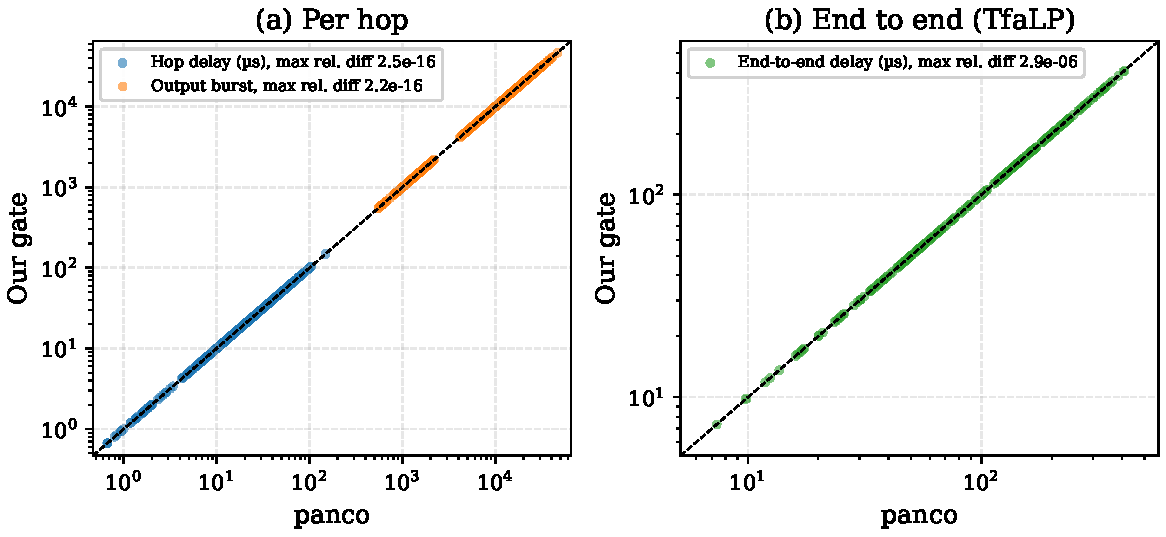
\includegraphics[width=\linewidth]{figures/panco_agreement.pdf}

\vspace{0.15cm}
\stattile{midblue}{$3.3\times10^{-16}$}{per hop, 837 values}
\hspace{0.2cm}
\stattile{tealblue}{$2.9\times10^{-6}$}{end to end, 210 values}

\vspace{0.05cm}
{\scriptsize max.\ relative difference (end to end: lp\_solve prints 6 digits)}
\end{columns}
\end{frame}

\begin{frame}{4. Results: Simulation and Admission Rate}
\small
\begin{columns}[T,totalwidth=\textwidth]
\column{0.49\textwidth}
\centering
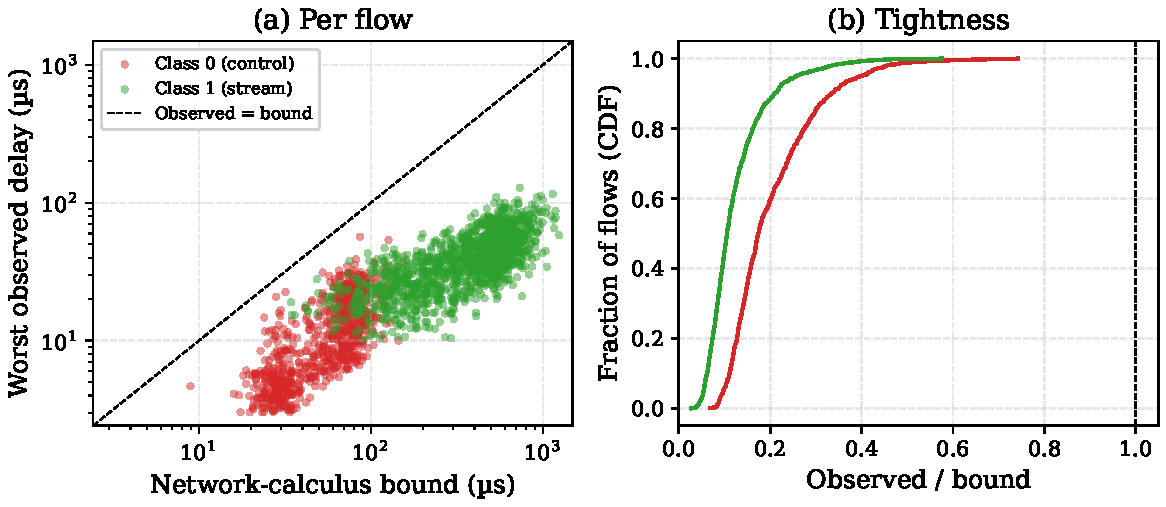
\includegraphics[width=\linewidth]{figures/bound_tightness.pdf}
\footnotesize
\textbf{0 violations} over 2,118 admitted flows; median observed/bound 0.17 (class 0), 0.11 (class 1). A sanity check, not a tightness measure.
\column{0.49\textwidth}
\centering
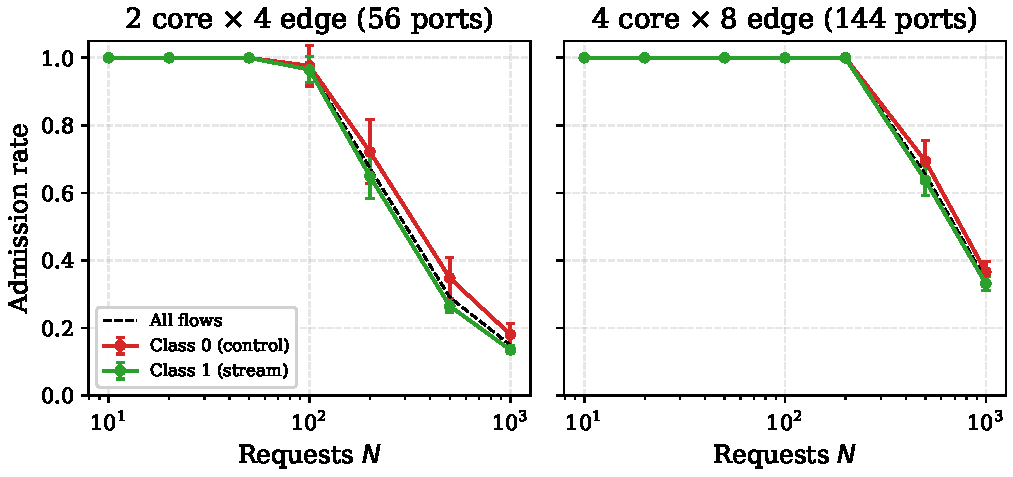
\includegraphics[width=\linewidth]{figures/admission_rate.pdf}
\footnotesize
All requests accepted up to $\approx$50; saturation at $100\pm20$ (line) and $111\pm16$ (tree) of 1,000; class 0 accepted slightly more often.
\end{columns}
\end{frame}

\begin{frame}{4. Results: Run Time of the Full and Incremental Gates}
\small
\begin{columns}[T,totalwidth=\textwidth]
\column{0.54\textwidth}
\centering
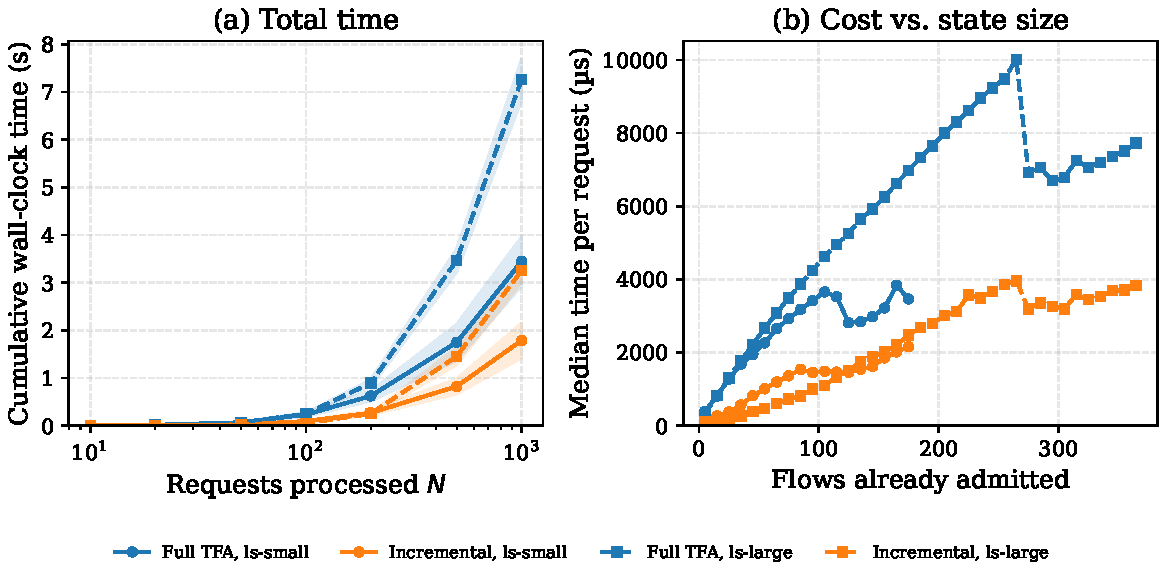
\includegraphics[width=\linewidth]{figures/scalability.pdf}
\column{0.44\textwidth}
\scriptsize
\centering
\begin{tabular}{llrr}
\toprule
Topology & Gate & Median $\mu$s & Speed-up \\
\midrule
Line & Full & 1944 & \\
     & Incremental & 964 & $2.02\times$ \\
Tree & Full & 2202 & \\
     & Incremental & 1186 & $1.91\times$ \\
\bottomrule
\end{tabular}
\vspace{0.3cm}
\begin{itemize}
  \item Identical verdicts and \textbf{bit-identical} bounds.
  \item Gain modest on small networks: a request still re-evaluates 19 of 48 ports (median).
  \item 18 unit tests, incl.\ tampered certificates (C5 and C0 reject them).
\end{itemize}
\end{columns}
\end{frame}

% ============================================================
\section{5. Limitations}
% ============================================================

\begin{frame}{5. Limitations}
\small
\begin{columns}[T,totalwidth=\textwidth]
\column{0.48\textwidth}
\begin{block}{Model}
Single link rate, fixed routing, feed-forward, strict NP-SP; no CBS/TAS shapers, preemption or clock effects; Ethernet overheads folded into $L_f,b_f,r_f$.
\end{block}
\begin{block}{Analysis}
TFA is sound but pessimistic compared with PMOO or LP-based analyses \cite{bondorf2014discodnc,bouillard2018dnc}: fewer admissions, never an unsafe one.
\end{block}
\column{0.48\textwidth}
\begin{block}{Certification}
Proof sketch on paper, not mechanised; floating-point checker with $10^{-9}$ tolerance; the certificate attests to the model, not to the deployed switches.
\end{block}
\begin{block}{Evaluation}
Additions only; small networks (saturation $\approx$100 flows), two classes; simulator does not force the worst case; no proposer connected yet.
\end{block}
\end{columns}
\end{frame}

% ============================================================
\section{6. Conclusion}
% ============================================================

\begin{frame}{6. Conclusion}
\small
\begin{columns}[T,totalwidth=\textwidth]
\column{0.48\textwidth}
\begin{block}{Contribution}
\footnotesize\raggedright
\begin{itemize}
  \item \textbf{Safe traffic allocation}: a flow is admitted only if every deadline still holds.
  \item \textbf{Certificate} per decision, re-checked by a 50-line checker (C0--C6).
  \item \textbf{Any proposer}, even a learned one, cannot commit an unsafe allocation.
  \item \textbf{Incremental gate}: $\approx$1\,ms, bit-identical bounds, 1.9--2.0$\times$ faster.
  \item \textbf{Validated}: matches panco; 0 violations over 2,118 flows.
\end{itemize}
\end{block}
\column{0.48\textwidth}
\begin{block}{Future directions}
\footnotesize\raggedright
\begin{itemize}
  \item \textbf{Capacity}: tighter, still checkable analyses than TFA.
  \item \textbf{Coverage}: CBS and TAS shapers, frame preemption.
  \item \textbf{Trust}: mechanised proof, exact-arithmetic checker.
  \item \textbf{Operations}: flow removal and batched changes.
  \item \textbf{Proposers}: the gate as a shield behind heuristic, ILP and DRL.
\end{itemize}
\end{block}
\end{columns}
\end{frame}

\begin{frame}[plain]
\begin{tikzpicture}[remember picture,overlay]
  \fill[gravyblue] (current page.south west) rectangle (current page.north east);
  \fill[softblue,opacity=.13] ($(current page.north west)+(1,-1)$) circle (3.1);
  \fill[midblue,opacity=.17] ($(current page.south east)+(-1,1)$) circle (3.4);
\end{tikzpicture}
\vspace{1.6cm}
\begin{center}
{\color{white}\Huge\bfseries Thank you for your attention!}\\[0.6cm]
{\color{softblue}\Large Questions?}
\end{center}
\end{frame}

\appendix

\begin{frame}[allowframebreaks]{References}
\nocite{*}
\scriptsize
\bibliographystyle{unsrt}
\bibliography{ref}
\end{frame}

\end{document}
